\documentclass[12pt]{article}

\usepackage[utf8]{inputenc}
\usepackage[T1]{fontenc}
\usepackage[polish,provide=*]{babel}
\usepackage{lmodern}
\usepackage{amsmath}
\usepackage{latexsym,amsfonts,amssymb,amsthm,amsmath}
\usepackage{enumitem}
\usepackage{hyperref}
\usepackage{float}
\usepackage{graphicx}
\usepackage{subcaption}
\usepackage{booktabs}
\graphicspath{{./images/}}

\setlength{\parindent}{0in}
\setlength{\oddsidemargin}{0in}
\setlength{\textwidth}{6.5in}
\setlength{\textheight}{8.8in}
\setlength{\topmargin}{0in}
\setlength{\headheight}{18pt}

\title{Przemiany Gazowe}
\author{Kacper Kłos}

\begin{document}

\maketitle

W poniższym raporcie przeanalizujemy zachowanie powietrza podczas dwóch przemian gazowych. Wpierw wykonywaliśmy przemianę izohoryczną w celu wyznaczenia temperatury zera bezwzględnego oraz liczbę moli obecną w badanym układzie. Z dwóch serii pomiarowych otrzymaliśmy temperatury \({T_0}_1 = (-287 \pm 8) ^\circ C\), \({T_0}_2 = (-282 \pm 6) ^\circ C\) oraz mole układu \(n_1 = (20{,}1\pm0{,}7) \times 10^{-3} mol\), \(n_2 = (20{,}2\pm0{,}5) \times 10^{-3} mol\), dając sumarycznie temperature zera bezwzględnego równą \(T_0 = (-284 \pm 5) ^\circ C\). Następnie wykonywaliśmy przemianę izotermiczną aby zbadać zakres poprawności równania gazu doskonałego i wyznaczyć liczbę moli w układzie. W dwóch seriach uzyskaliśmy zakresy ciśnień \(P_1 \in [105{,}5; 152{,}1] \, kPa\) i \(P_2 \in [60{,}7; 97{,}6] \, kPa\) przy liczbie moli \(n_1 = (4{,}4\pm0{,}7) \times 10^{-3} mol\), \(n_2 = (1{,}5\pm0{,}5) \times 10^{-3} mol\).

\newpage
\section{Analiza Wyników}
\subsection{Czujniki i stałe}
W obu pomiarach będziemy korzystać z czujników ciśnienia PASCO PS-3203\cite{pressure} o dokładności 2 kPa oraz czujnika temperatury PASCO PS-3222\cite{temperature} z błędem 0{,}5 \(^\circ C\). Podczas wyznaczania wartości będziemy wykorzystywać stałą gazową\cite{gas_const} \(R = 8{,}314 \, mol^{-1} K^{-1}\).
\subsection{Przemiana Izohoryczna}
Pomiary zaczynamy od przemiany izohorycznej, gdzie w miedzianej sferze o promieniu 2 cali szczelnie zamknięta jest stała liczba moli powietrza. Wewnątrz sfery zawarte są wspomniane czujniki które pozwalają nam mierzyć temperature i ciśnienie. Sfere nagrzewamy w izolowanym pojemniku na wode lejąc na nią wrzątek z czajnik i czekając aż gaz osiągnie równowage termodynamiczną.

\begin{table}[H]
    \centering
    \begin{tabular}{c|cc|cc}
        \toprule
        \textbf{Nr} & $T_1 \, [^\circ$C] & $P_1 \, [kPa]$ & $T_2 \, ^\circ$C] & $P_2 \,[kPa]$ \\
        \midrule
        1  & 5{,}9   & 95{,}1  & 7{,}9   & 87{,}6  \\
        2  & 12{,}7  & 97{,}4  & 18{,}0  & 91{,}2  \\
        3  & 17{,}2  & 98{,}9  & 27{,}0  & 94{,}1  \\
        4  & 23{,}6  & 100{,}6 & 31{,}2  & 95{,}6  \\
        5  & 29{,}6  & 102{,}7 & 37{,}1  & 98{,}3  \\
        6  & 34{,}7  & 104{,}9 & 40{,}7  & 99{,}1  \\
        7  & 40{,}1  & 106{,}5 & 47{,}5  & 100{,}7 \\
        8  & 46{,}3  & 108{,}1 & 50{,}3  & 101{,}4 \\
        9  & 52{,}3  & 108{,}9 & 53{,}9  & 102{,}6 \\
        10 & 58{,}5  & 110{,}6 & 57{,}5  & 103{,}8 \\
        11 & 64{,}0  & 113{,}8 & 60{,}9  & 104{,}6 \\
        12 & 71{,}1  & 114{,}9 & 65{,}6  & 105{,}8 \\
        13 & 79{,}4  & 119{,}4 & 70{,}0  & 106{,}9 \\
        14 & 84{,}8  & 122{,}1 & 75{,}4  & 109{,}3 \\
        15 & --     & --      & 81{,}6  & 110{,}2 \\
        \bottomrule
    \end{tabular}
    \caption{Pomiary izochoryczne: ciśnienie $P$ z błędem $2 \, kPa$ oraz temperatury $T$ z błędem $0{,}5 ^\circ C$ dla dwóch serii pomiarowych.}
    \label{tab:isochoric_measurements}
\end{table}


Przy pomocy otrzymanych danych jesteśmy w stanie oszacować temperature oraz liczbę moli zera bezwzględnego, zakładając że gaz w badanym zakresie zachowuje się jak gaz doskonały opisywany równaniem\cite{skrypt}:
\[
    PV = nR(T - T_0)
\]
Gdzie \(P\), \(V\), \(n\), \(R\), \(T\), \(T_0\) oznaczają kolejno mierzone ciśnienie, objętośc gazu, liczba moli, stała gazowa, mierzona temperatura oraz temperatura zera bezwzględnego. Możemy zauważyć że niepewność ciśnienia na poziomie 2kPa oznacza okolice 2\% wartości naszych pomiarów ciśnienia, gdy błąt pomiaru temperatury na poziomie 0{,}5 \(C^\circ\)zaczyna się od około 2\%, lecz szybko maleje aż do 0{,}2\%. Wskazuje to że pomiar temperatury jest znacznie dokładniejszy, dlatego parametry będziemy dopasowywać do równania:
\[
    P = aT + b
\]
W ten sposób za pomocą danych z tab.~\ref{tab:isochoric_measurements} otrzymujemy wykresy:
\begin{figure}[H]
    \centering
    \begin{subfigure}{0.47\textwidth}
        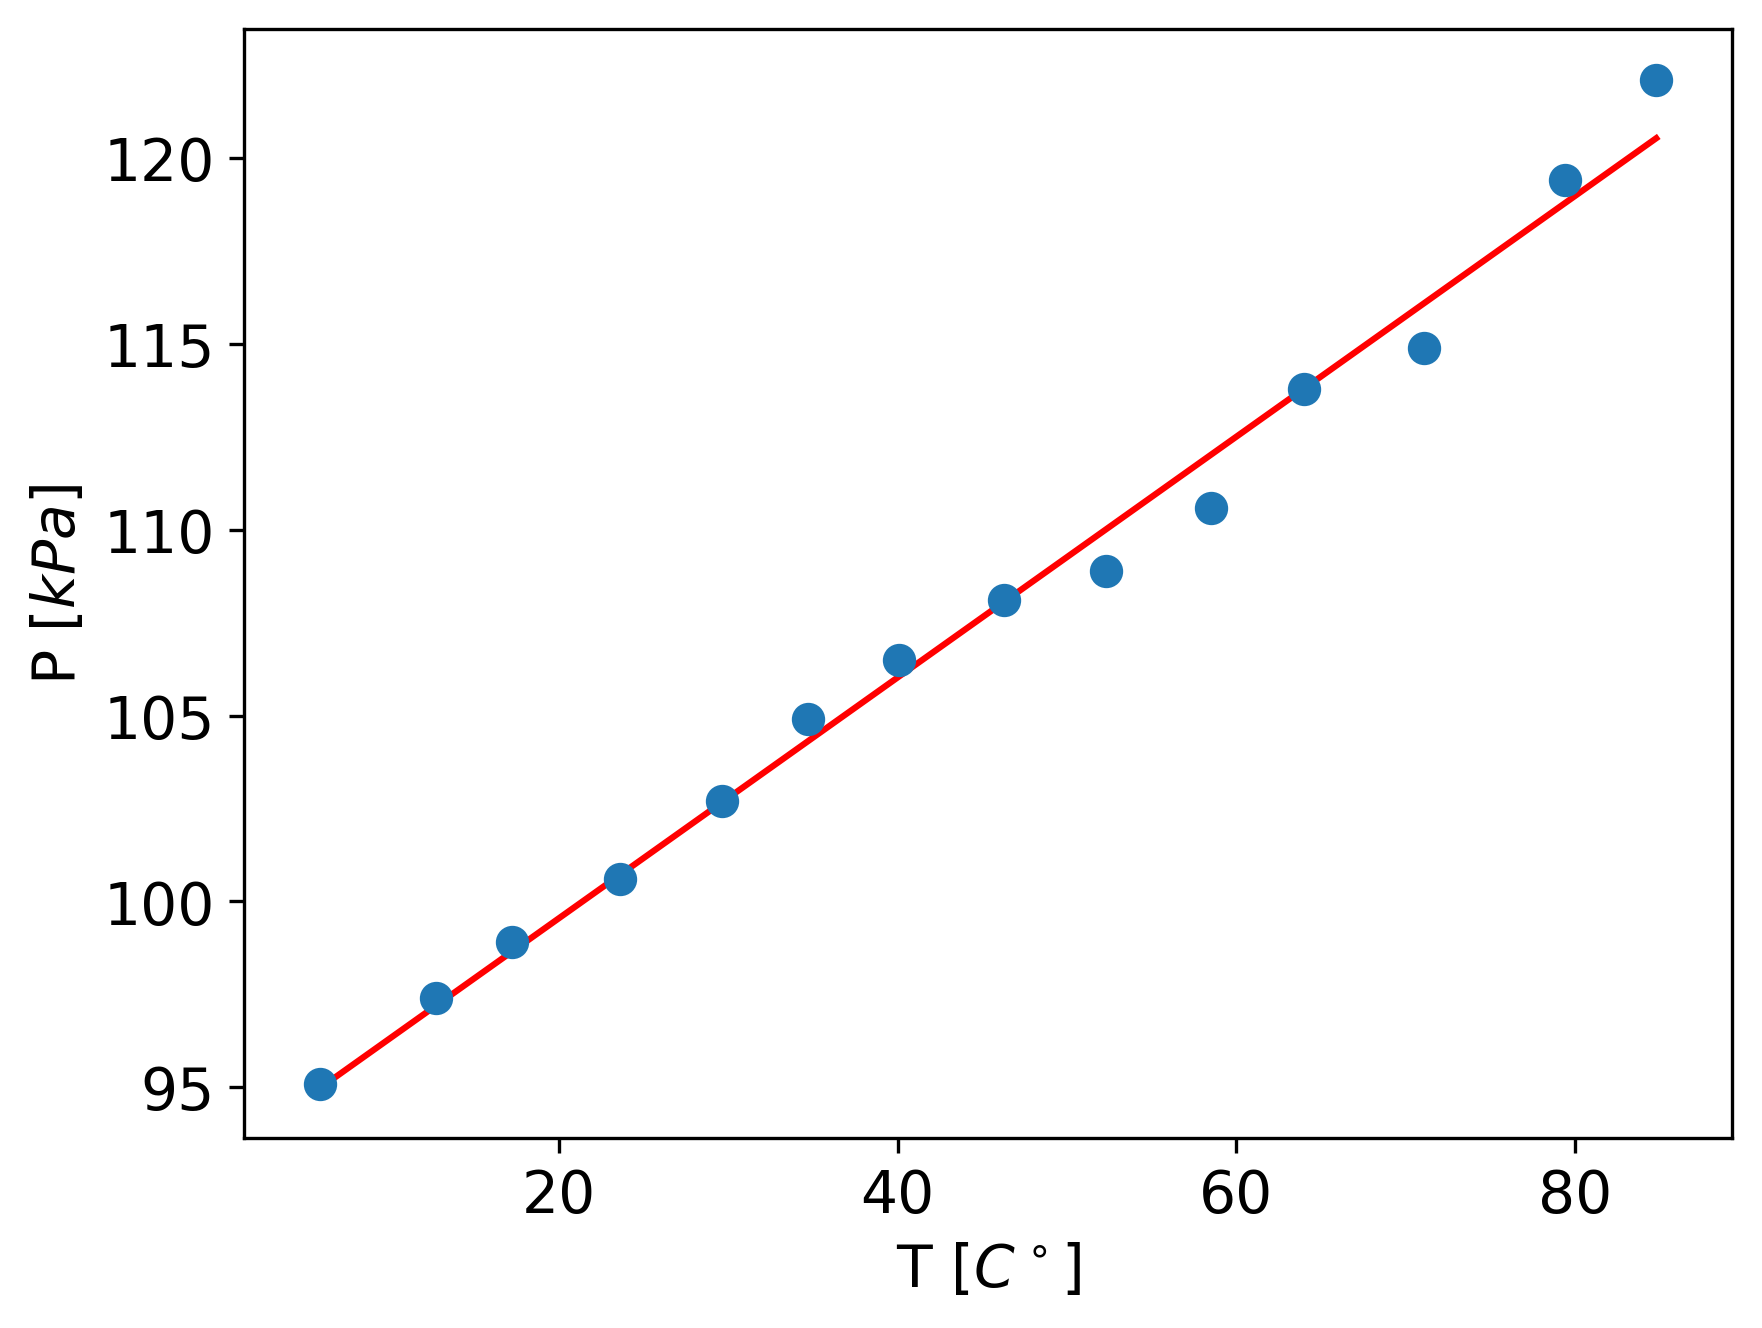
\includegraphics[width=\linewidth]{izohoric_0}
        \caption{1 seria pomiarowa}
    \end{subfigure}\hfill
    \begin{subfigure}{0.47\textwidth}
        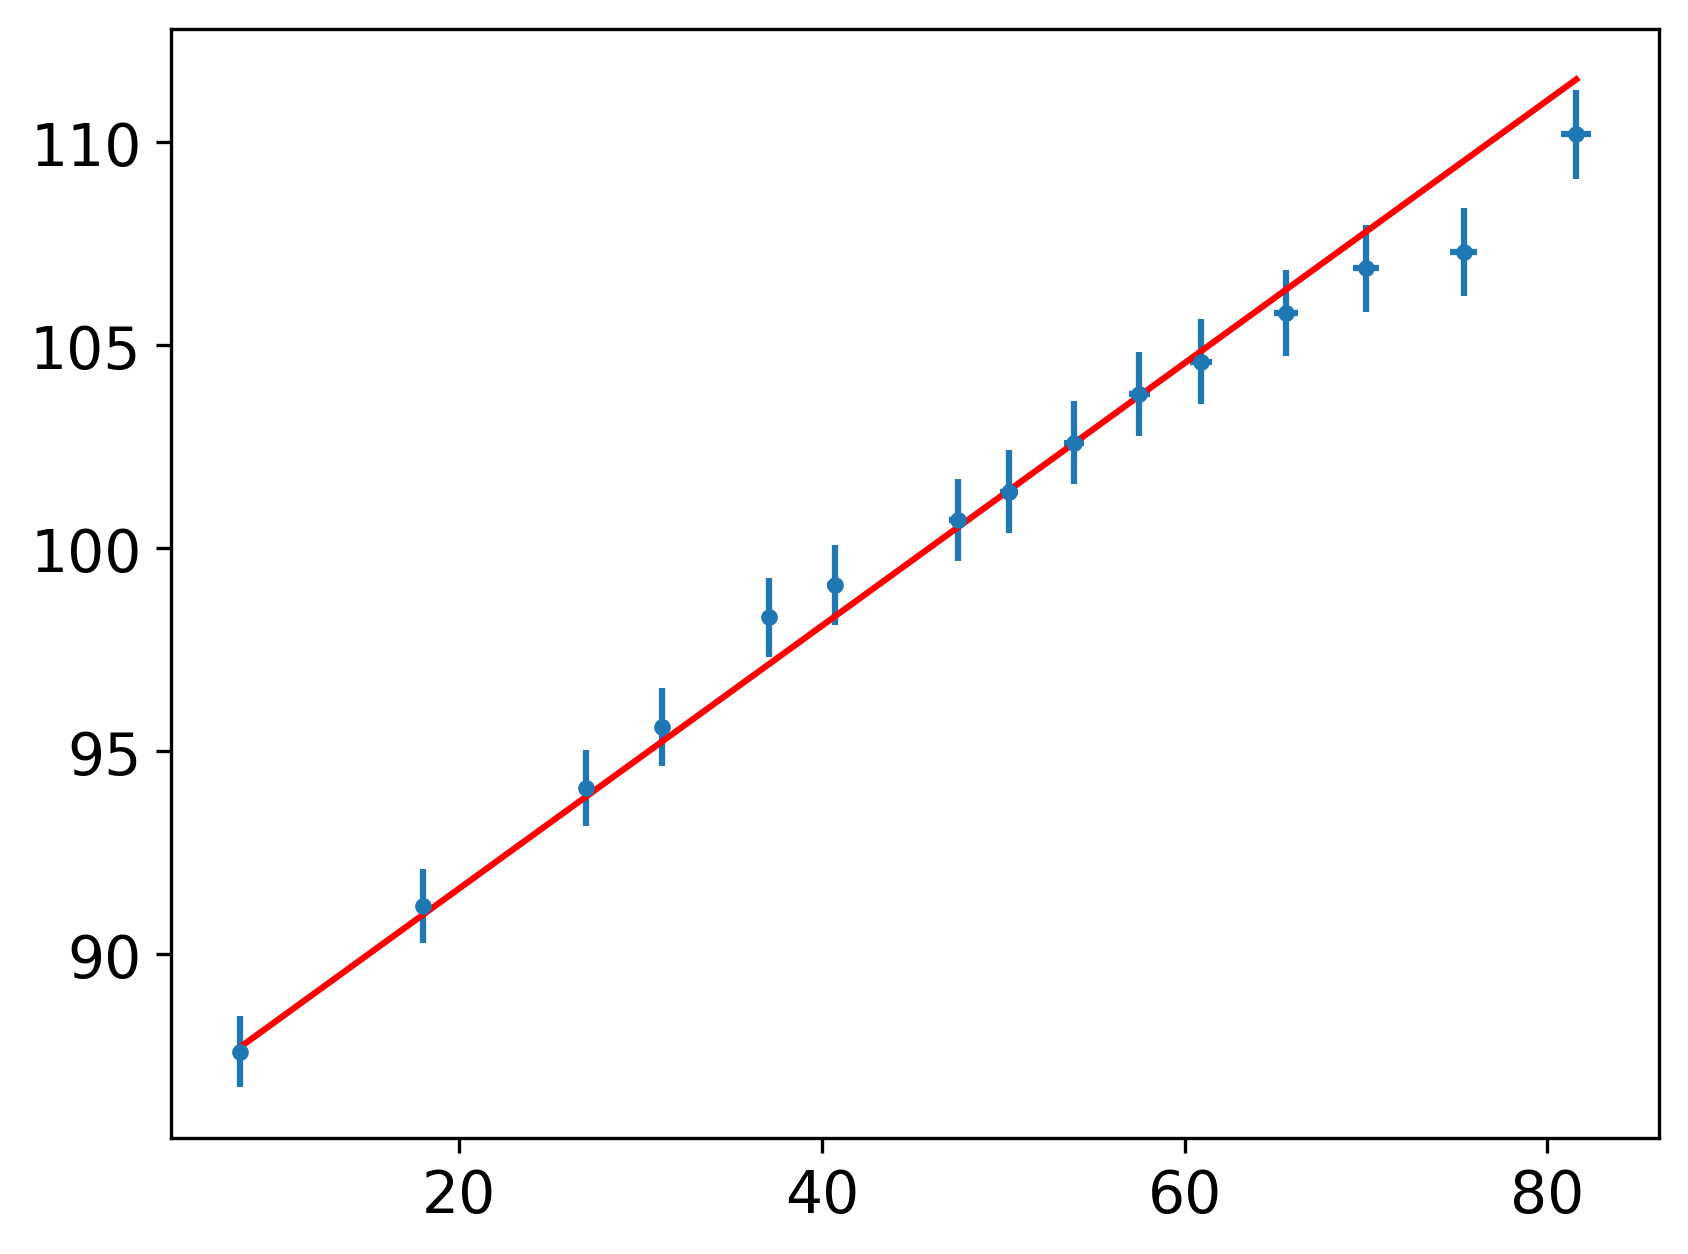
\includegraphics[width=\linewidth]{izohoric_1}
        \caption{2 seria pomiarowa}
    \end{subfigure}
    \caption{Zależność ciśnienia \(P\) od temperatury \(T\) podczas ogrzewania powietrza w miedzianej kuli o stałej objętości \(V\)}
    \label{fig:izohoric}
\end{figure}
Gdzie parametry wynoszą
\[
    a_1 = (0{,}32 \pm 0{,}01) \, kPa \, (^\circ C)^{-1}, \quad b_1 = (93{,}1 \pm 0{,}5) \, kPa
\]
\[
    a_2 = (0{,}305 \pm 0{,}06)  \, kPa \, (^\circ C)^{-1}, \quad b_2 = (85{,}99 \pm 0{,}32) \, kPa
\]
Z tych parametrów możemy otrzymać temperature zera bezwzględnego i liczbę moli
\[
    T_0 = -\frac{b}{a}, \quad n = \frac{aV}{R}
\]
Co przy użyciu standardowego wzoru na objętość sfery przy promieniu 2 cali (1 cal = 2{,}54 cm) i wspomnianej już wartości stałej \(R\) skutkuje:
\[
    {T_0}_1 = (-287 \pm 8) \, ^\circ C, \quad n_1 = (20.1 \pm 0.7) \times 10^{-3} \, mol
\]
\[
    {T_0}_2 = (-282 \pm 6) \, ^\circ C, \quad n_2 = (20.2 \pm 0.5) \times 10^{-3} \, mol
\]
Z średniej ważonej otrzymujemy temperature
\[
    T_0 = (-284 \pm 5) \, ^\circ C
\]
\subsection{Przemiana Izotermiczna}
W tej części mierzyliśmy ciśnienie, temperature i objętość powietrzaw w strzykawce za podłączonymi wspomnianymi wyżej czujnikami ciśnienia oraz temperatury. Do końca strzykawki podłączyliśmy przewody które podpieliśmy do czujników, następnie przesówając tłok strzykawki zmienialiśmy objętość powietrza następnie czekając aż temperatura wróci do temperatury otoczenia.

\begin{table}[H]
    \centering
    \begin{tabular}{c|cc|cc}
        \toprule
        \textbf{Nr} &
        $V_1$ [mL] & $P_1$ [kPa] &
        $V_2$ [mL] & $P_2$ [kPa] \\
        \midrule
        1  & 60 & 99{,}6  & 26 & 97{,}6  \\
        2  & 56 & 105{,}5 & 30 & 87{,}4  \\
        3  & 52 & 110{,}4 & 34 & 78{,}8  \\
        4  & 48 & 116{,}0 & 38 & 73{,}1  \\
        5  & 44 & 121{,}1 & 42 & 68{,}0  \\
        6  & 41 & 125{,}3 & 46 & 63{,}9  \\
        7  & 37 & 130{,}5 & 50 & 60{,}7  \\
        8  & 33 & 137{,}7 & 54 & 57{,}9  \\
        9  & 29 & 144{,}8 & 58 & 56{,}3  \\
        10 & 26 & 152{,}1 & 60 & 55{,}6  \\
        \bottomrule
    \end{tabular}
    \caption{Pomiary objętości $V$ z niepewnością $1{,}2 \, mL$ oraz ciśnienia $P$ z niewpewnością $2 \, kPa$ dla gazu zawartego w strzykawce przy stałej temperaturze $23{,}0 \pm 0{,}1 ^\circ C$ dla dwóch serii pomiarowych.}
    \label{tab:syringe_data_with_updated_values}
\end{table}


Przy pomocy tych danych postaramy się oszacować w jakim zakresie powietrze zachowuje się jak gaz doskonały wyznaczając zależność:
\[
    \frac{P(V + V_0)}{T - T_0} = nR = \text{const}
\]
Gdzie symbole mają to samo znaczenie co w poprzedniej sekcji oraz \(V_0\) oznacza objętość powietrza zawartą w przewodach z gazem. W pomiarach dążyliśmy do tego aby temperatura pozosawała stale w okolicach \(T = (23{,}0 \pm 0{,}1) \, ^\circ C\). Przekształcając to równanie na zależne od ciśnienia możemy zbadać zakres poprawności założenia że powietrze jest gazem doskonałym oraz wyznaczyć liczbę moli. Jako temperature zera bezwzględnego\cite{zero} przyjmujemy \(T_0 = -273{,}15\,C^\circ\).
\[
    \frac{PV}{T - T_0} = aP + b
\]
Wyliczając te zależności otrzymujemy wykresy \ref{fig:izotermic} i ich dopasowania liniowe do danych z tab.~\ref{tab:syringe_data_with_updated_values} dla zakresów w którch zauważalna była zależność liniowa:
\begin{figure}[H]
    \centering
    \begin{subfigure}{0.47\textwidth}
        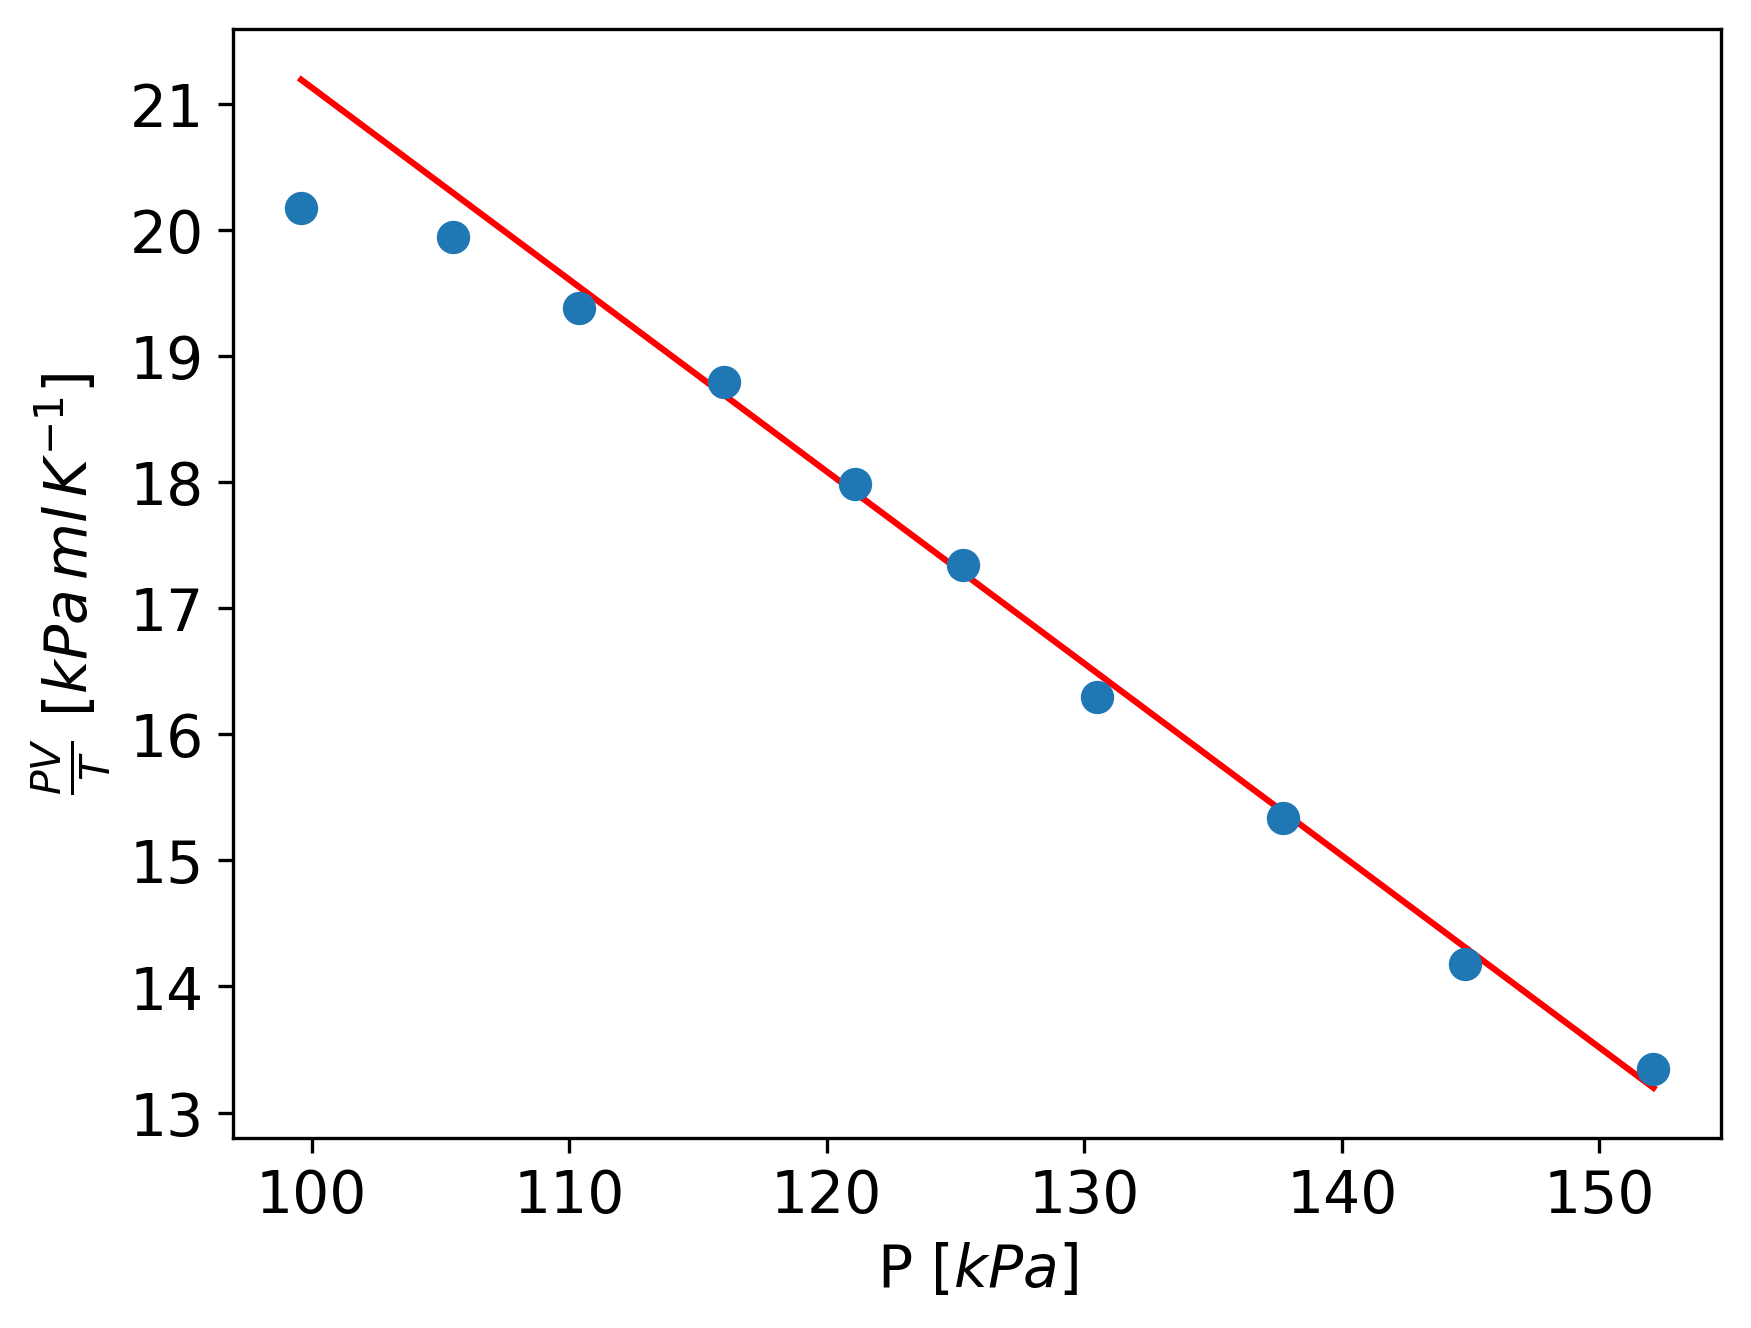
\includegraphics[width=\linewidth]{izotermic_0}
        \caption{1 seria pomiarowa, sprężanie}
    \end{subfigure}\hfill
    \begin{subfigure}{0.47\textwidth}
        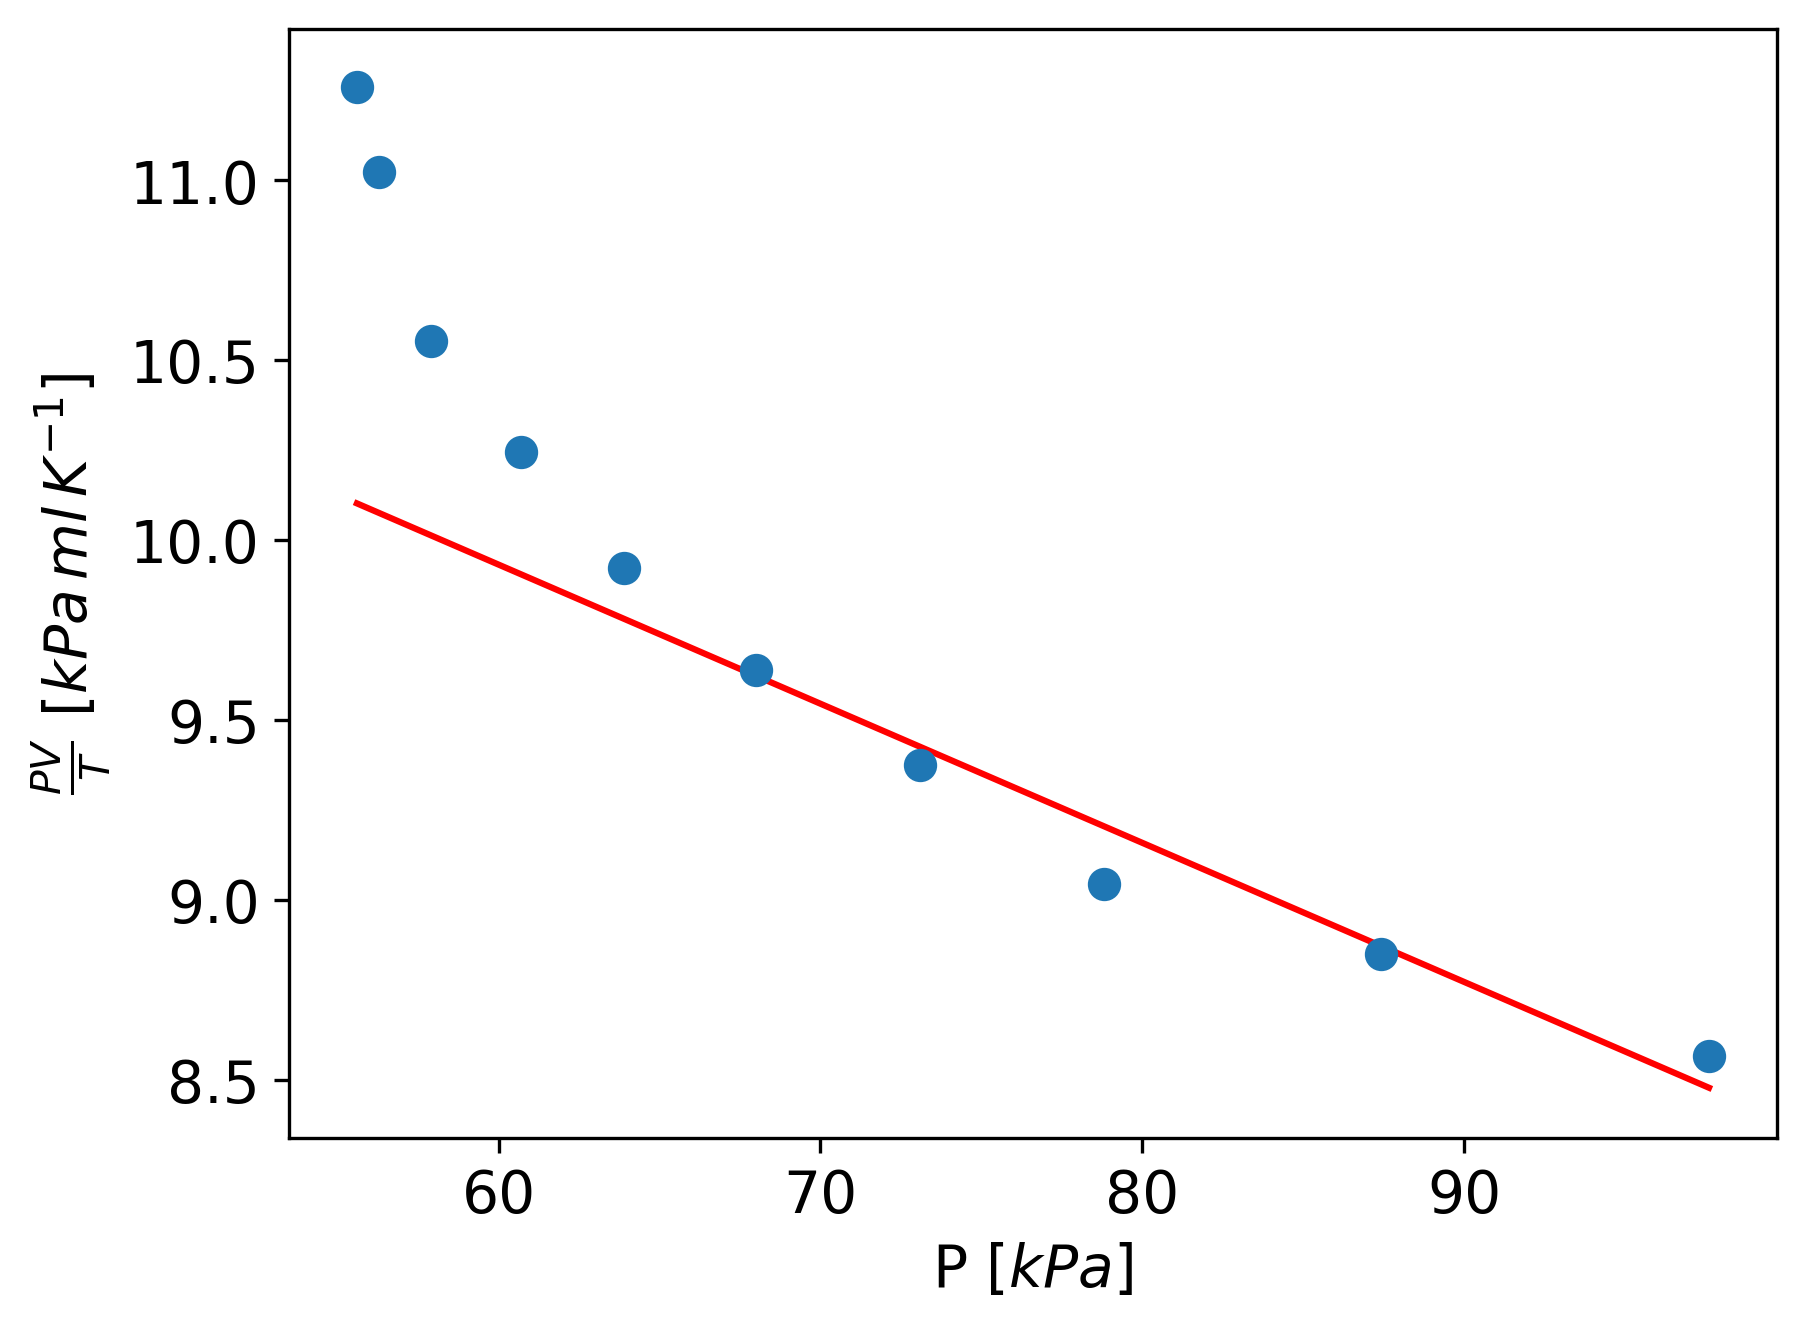
\includegraphics[width=\linewidth]{izotermic_1}
        \caption{2 seria pomiarowa, rozprężanie}
    \end{subfigure}
    \caption{Wykres zależności \(\frac{PV}{T + T_0}\) od ciśnienia \(P\) przy stałej temperaturze \(T = (23{,}0 \pm 0{,}1) \, ^\circ C\) dla dwóch różnych ilości moli zawartych w strzykawce.}
    \label{fig:izotermic}
\end{figure}
Z wykresu odczytujemy zakres w którym aplikuje się równanie gazu doskanałego jako punkty które z błędem dotykają dopasowania liniowego
\[
    P_1 \in [105{,}5; 152{,}1] \, kPa, \quad P_2 \in [60{,}7; 97{,}6] \, kPa,
\]
Gdzie w zakresach liniowych otrzymujemy parametry:
\[
    a_1 = (-0{,}154 \pm 0{,}005) \, mL K^{-1}, \quad b_1 = (36{,}6 \pm 0{,}6) \, Pa L K^{-1}
\]
\[
    a_2 = (-0{,}040 \pm 0{,}005) \, mL K^{-1}, \quad b_2 = (12{,}33 \pm 0{,}34) \, Pa L K^{-1}
\]

Za ich pomocą i wspomnianej wartości \(R\) możemy wyznaczyć liczbę moli:
\[
    n = \frac{b}{R}
\]
\[
    n_1 = (4{,}4 \pm 0{,}7) \times 10^{-3} \, mol ,\quad n_2 = (1{,}5 \pm 0{,}5) \times 10^{-3} \, mol
\]

\newpage

\section{Podsumowanie}
Widzimy że otrzymana temperatura zera bezwzględnego \(T_0 = (-284 \pm 5) \, ^\circ C\) zawiera w swoim przedziale \(3 \sigma\) profesjonalnie wyznaczoną temperature\cite{temperature} \(T_0 = -273{,}15\,C^\circ\). Głównym problemem jaki napotkaliśmy podczas jej wyznaczania jest problem z ustaleniem kiedy nastała równowaga. Szczególnie w przypadku wyższych temperatur trudno było określić czy spadak wynika z naturalnego chłodzenia się układu lub czy sfera była miejscowo nagrzana przy czujniku i trzeba czekać aż dojdzie do równowagi. Podczas pomiarów izotermicznych możemy zauważyć że przedział aplikowalności równania gazu doskonałego znacznie zmienia się wraz z liczbą moli, dla układu z \(n_1 = (4{,}4 \pm 0{,}7) \times 10^{-3} \, mol\) otrzymaliśmy przedział \(P_1 \in [105{,}5; 152{,}1] \, kPa\), podczas gdy liczba moli \(n_2 = (1{,}5 \pm 0{,}5) \times 10^{-3} \, mol\) odpowiada przedziałowi \(P_2 \in [60{,}7; 97{,}6] \, kPa\). Co ciekawe liczba moli miała też znaczny wpływ na to w jaki sposób załamywało się to równanie, przy dużej liczbie moli wykres miał ujemną krzywiznę w przeciwieństwie do małej liczby w której miał dodatni. Główną przyczyną błędów w tych pomiarach był nieszczelny układ, po zmianie odległości można było zauważyć stały dryf ciśnień w kierunku ciśnienia otoczenia co przeszkadzało w określeniu kiedy układ był w równowadze oraz mogło mięc znaczący wpływ na ostatnie pomiary w serii kiedy ten błąd skumujował się z wszytkich poprzednich punktów.

\begin{thebibliography}{5}

    \bibitem{temperature}
    \url{https://cdn.pasco.com/product_document/Wireless-Temperature-Link-Manual-PS-3222_1_.pdf}
    \bibitem{pressure}
    \url{https://www.pasco.com/products/sensors/wireless/wireless-pressure-sensor#documents-panel}
	\bibitem{skrypt}
	\emph{BADANIE PRZEMIAN GAZOWYCH, WYZNACZANIE TEMPERATURY ZERA BEZWZGLĘDNEGO}, Aneta Drabińska, Uniwersytet Warszawski.
    \bibitem{gas_const}
    \url{https://physics.nist.gov/cgi-bin/cuu/Value?r}
    \bibitem{zero}
    \url{https://www.bipm.org/documents/20126/41483022/SI-Brochure-9-EN.pdf/2d2b50bf-f2b4-9661-f402-5f9d66e4b507}

\end{thebibliography}


\end{document}
